\begin{frame}
  \frametitle{Restbudget}

  \begin{columns}
    \column{0.7\linewidth}
      \begin{figure}
        \centering
		    \only<1|handout:0>{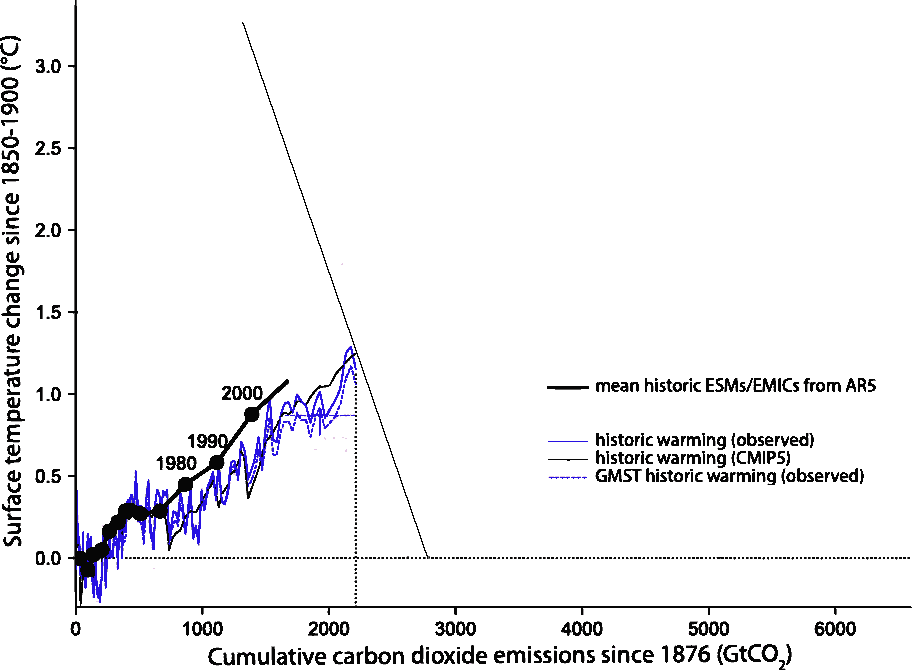
\includegraphics[trim={0cm 0.cm 0cm 0cm}, clip, width=\linewidth]{bilder/cumulative_co2/cumulative_co2-1.pdf}}
        \only<2|handout:0>{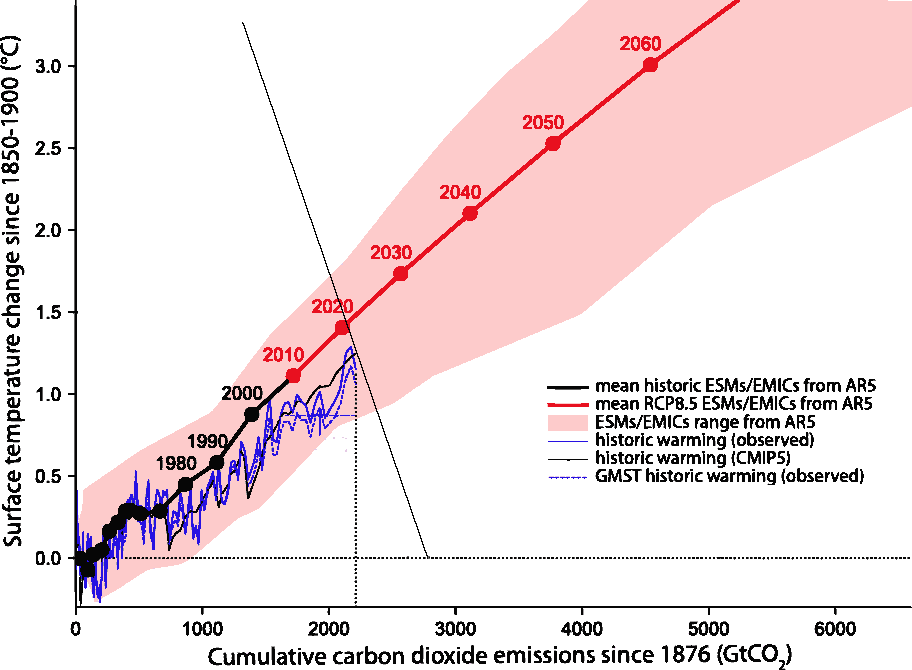
\includegraphics[trim={0cm 0.0cm 0cm 0cm}, clip, width=\linewidth]{bilder/cumulative_co2/cumulative_co2-2.pdf}}
        \only<3|handout:0>{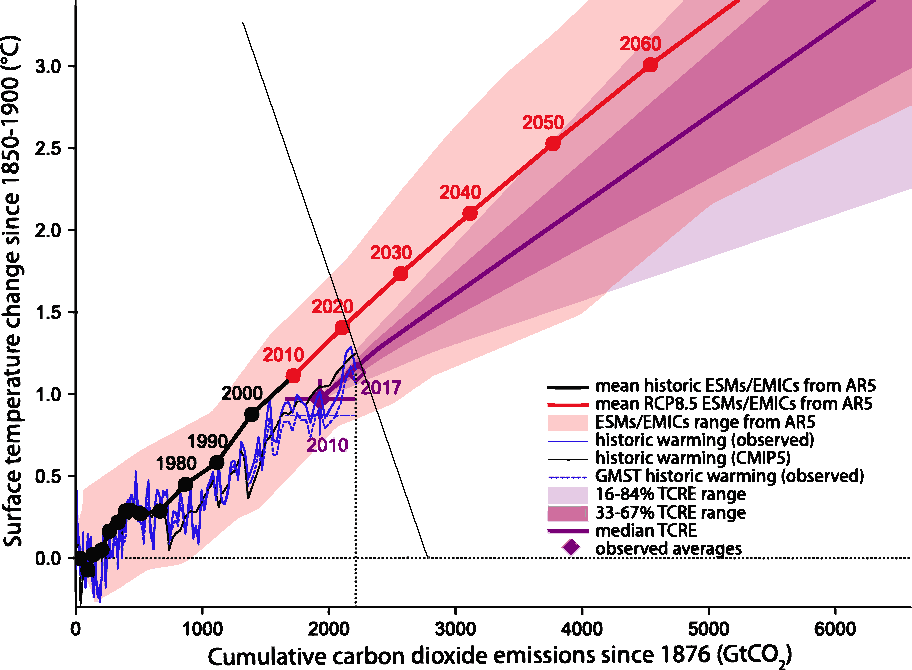
\includegraphics[trim={0cm 0.0cm 0cm 0cm}, clip, width=\linewidth]{bilder/cumulative_co2/cumulative_co2-3.pdf}}
        \only<4-5|handout:1>{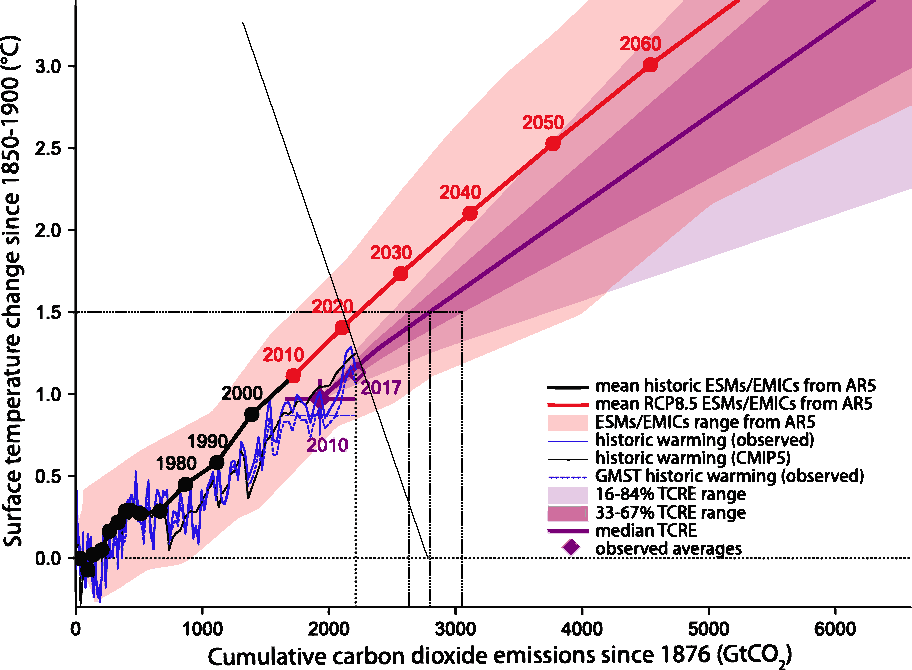
\includegraphics[trim={0cm 0.0cm 0cm 0cm}, clip, width=\linewidth]{bilder/cumulative_co2/cumulative_co2-4.pdf}}
        \vspace{-0.5cm}
		    \caption{Globale Oberflächentemperatur gegen kumulative CO$_2$-Emissionen. Quelle: IPCC 2018, Kapitel 2}
      \end{figure}
    \column{0.3\linewidth}
    \only<1|handout:0>{
      \begin{itemize}
        \item[] Temperaturerhöhung gegen kumulierte CO$_2$-Emissionen
      \end{itemize}
    }
    \only<2|handout:0>{
      \begin{itemize}
        \item[] \enquote{business-as-usual}
        \item[$\rightarrow$] RCP8.5 Szenario des IPCC
      \end{itemize}
    }
    \only<3|handout:0>{
      \begin{itemize}
        \item[2010] \SI{0.97}{\degreeCelsius} Erwärmung und
                    \SI{1930}{\GtCO} Emissionen
        \item[2017] \SI{1.10}{C} Erwärmung und
                    \SI{2220}{\GtCO} Emissionen
      \end{itemize}
    }
    \only<4-|handout:1>{
      \begin{itemize}
        \item[\num{420}] \GtCO Restbudget $\rightarrow$ \SI{1.5}{\degreeCelsius} mit \SI{66}{\%}iger Wahrscheinlichkeit
        \item[\num{580}] \GtCO Restbudget $\rightarrow$ \SI{1.5}{\degreeCelsius} mit \SI{50}{\%}iger Wahrscheinlichkeit
        \item[\num{840}] \GtCO Restbudget $\rightarrow$ \SI{1.5}{\degreeCelsius} mit \SI{33}{\%}iger Wahrscheinlichkeit
        \item<5> Globale Emissionen in 2019 49 GtCO$_2$ % https://edgar.jrc.ec.europa.eu/overview.php?v=booklet2019
        \item<5>[$\Rightarrow$] Bei gleichbleibender Rate sind die Restbudgets in 8,5 bzw. 11,8 Jahren aufgebraucht
      \end{itemize}
    }
    \end{columns}

    \note<1-4>{
    \vspace{-2em}
      Abbildung aus dem Special Report 15 des IPCC von 2018, schrittweise erklärt
      \begin{itemize}
        \item Veränderungen der globalen Oberflächentemperatur gegen kumluative CO$_2$-Emissionen
        \item Dünne blaue Linie zeigt jährliche gemessene Werte.
        \item gestrichelte blaue Linie zeigt die mittlere globale Oberflächentemperatur.
        \item Schwarze Punkte und Linie zeigen mittels RCP8.5 reproduzierte historische Werte (20 ESMs/EMICs).
        \item Dünne schwarze Linie zeigt Rekonstruktion mittels der CMIP5 Modelle (41 Modelle vom letzten Mal).
      \end{itemize}
      }
      \note<2-4>{
      \begin{itemize}
        \item Rote Punkte und Linie: Vorhersagen des RCP8.5 Szenarios, Klimamodelle aus AR5 Bericht (20 ESMs/EMICs)
        \item Orangene Fläche zeigt die Bandbreite der Ergebnisse der im AR5 Bericht betrachteten Klimamodelle
      \end{itemize}
      }
      \note<3-4>{
      \begin{itemize}
        \item Lila Punkte und Flächen zeigen die Ergebnisse der im SR15 verwendeten Modelle und Daten (TCRE)
        \item Gefüllte lila Raute zeigt den Wert Ende 2010 mit einer Erwärmung von \SI{0.97}{\degreeCelsius} und \SI{1930}{\GtCO}
        \item Leere lila Raute zeigt den Wert Ende 2017 mit einer Erwärmung von \SI{1.10}{\degreeCelsius} und \SI{2220}{\GtCO}
      \end{itemize}
      }
      \note<4>{
      \begin{itemize}
        \item Gestrichelte Linien zu den Achsen zeigen die Menge kumulativer CO$_2$-Emissionen für eine Erwärmung von \SI{1.5}{\degreeCelsius}, aus denen sich Restbudgets für verbleibende Emissionen ableiten lassen
      \end{itemize}
      }
      \note<1-4>{
      \vfill
      \vspace{-0.5em}
      \begin{itemize}
        \item[AR5] Fifth Assessment Report des IPCC aus 2014, \enquote{Synthesis Report: Climate Change 2014}.
        \item[ESM] Earth System Models. Klimamodelle zur Beschreibung und Vorhersage des Erdklimas.
        \item[EMIC] Earth System Models of Intermediate Complexity. Modellerweiterungen für einzelne spezifische Fragestellungen wie die Entwicklung von Rückkopplungseffekten auf langen Zeitskalen.
        \item[CMIP5] Coupled Model Intercomparison Projects. Zusammenfassung einer Reihe an Klimamodellen.
        \item[GMST] Global mean surface temperature.
        \item[TCRE] Transient climate response to cumulative carbon emissions. Global Änderung der Oberflächentemperatur pro emittierter Einheit Kohlendioxid.
      \end{itemize}
    }
	\note<5>{
		\begin{itemize}
      \item Mögliche Reduktion um 100 GtCO$_2$ bei Berücksichtigung von Erdsystem-Rückkopplungen wie Auftauen von Permafrostböden
			\item Restbudgets einerseits aus Erwärmung im Vergleich zu 1861-1880 auf Basis des RCP8.5 Szenarios
      \item Andererseits \enquote{from a set of available pathways that were assessed to have a >50\% probability to exceed 1.5°C by mid-century, and return to 1.5°C or below in 2100 with greater than 66\% probability}
      \item Weitere Studien, die teilweise nur CO$_2$ berücksichtigen
      \item Seit dem AR5 Report 2014 viele weitere Veröffentlichungen, die berücksichtigt werden
      \item Viele Unsicherheiten auf die berechneten Restbudgets wie Unterschiede in Szenarien zur Entwicklung von nicht-CO$_2$ Emissionen oder die Unsicherheit auf die historische Temperatur von 1850-1900
      \item[$\Rightarrow$] Viele Unsicherheiten, aber dennoch: Die Zeit ist knapp!
		\end{itemize}
    Fragen?
	}
\end{frame}

\begin{frame}
  \frametitle{CO$_2$-Emissionen Deutschlands}
  \begin{columns}
    \column{0.7\linewidth}
      \begin{figure}
		    \centering
		    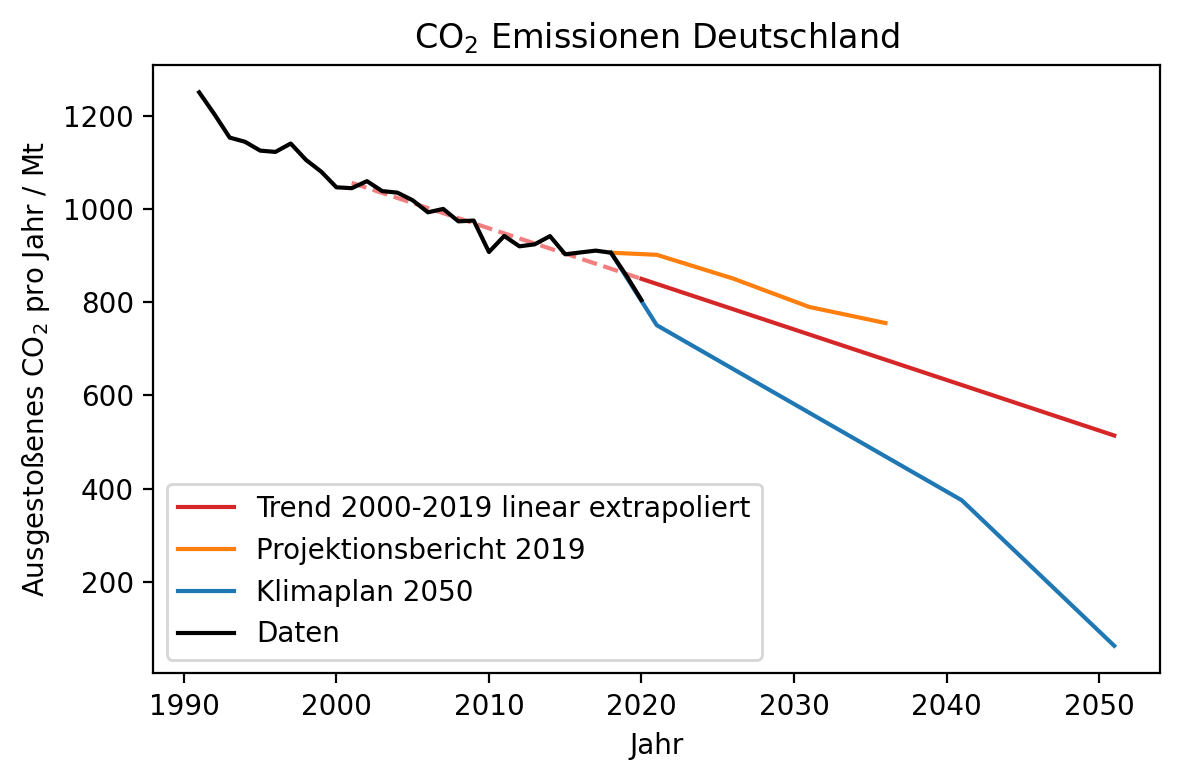
\includegraphics[width=\linewidth]{bilder/co2-emissions-de.png}
		    \caption{Szenarien der jährlichen CO$_2$-Emissionen Deutschlands.}
      \end{figure}
    \column{0.3\linewidth}
      \begin{itemize}
        \item Linearer Trend: Null-Emissionen in 80 Jahren.
        \item Bisherige Maßnahmen reichen nicht zur Erreichung der gesetzten Ziele.
        \item Klimaplan 2050 (Pariser Abkommen) zeigt ambitionierten Weg.
        \item[$\rightarrow$] Unklar, wie dieser Weg gegangen werden soll.
      \end{itemize}
    \end{columns}
    \note{
      \begin{itemize}
        \item[] Jährliche CO$_2$-Emissionen Deutschlands (schwarz)
        \item[] Linare Extrapolation des Trends aus den Jahren 2000-2019 (rot)
        \item[] Erwartete jährliche Emissionen aus dem Projektionsbericht 2019 der Bundesregierung auf Basis der zu dem Zeitpunkt beschlossenen oder vorbereiteten Maßnahmen (orange)
        \item[] Ziele des Klimaplans 2050 der Bundesregierung (blau)
      \end{itemize}
    }
\end{frame}

\begin{frame}
  \frametitle{Wie viele Emissionen stehen Deutschland noch zu?}
  \begin{columns}
    \column{0.7\linewidth}
      \begin{figure}
		    \centering
		    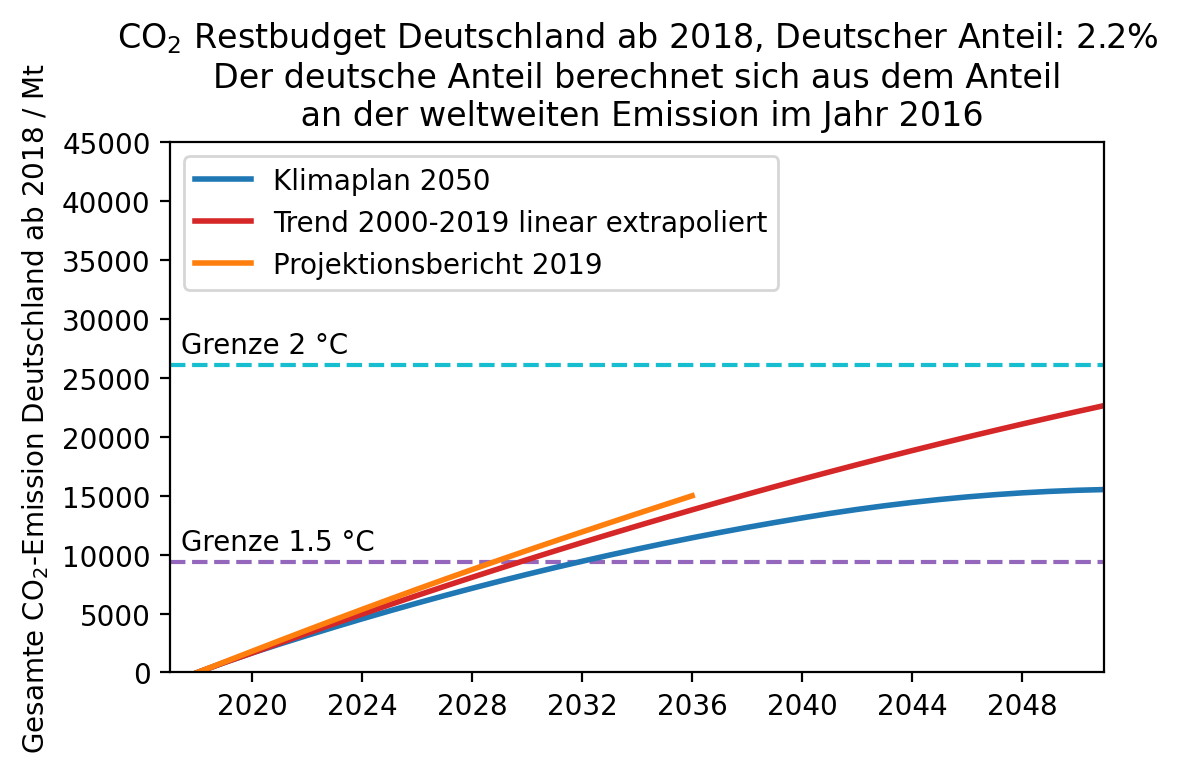
\includegraphics[width=1.05\linewidth]{bilder/restbudget_de_new.png}
		    \caption{Szenarien der kumulativen CO$_2$-Emissionen Deutschlands. \href{https://s4f-dortmund.github.io/pitch/2019/07/05/pitch.html}{\color{blue}\underline{S4F-Pitch}}}
      \end{figure}
    \column{0.3\linewidth}
      \begin{itemize}
        \item Emissionen 2016: 2,2\,\%
        \item Faire Verteilung: 1,1\,\%
        \item[$\rightarrow$]Trotz ungerechter Verteilung Überschreitung der Grenzen für 1,5°C
      \end{itemize}
    \end{columns}
    \note{
      \begin{itemize}
        \item[] Gleiche Datenlage wie für die vorherige Abbildung, allerdings wurden die jährlichen Emissionen kumuliert.
        \item[] CO$_2$-Restbudgets für 1.5°C und 2°C (66\%-ige Wahrscheinlichkeit) unter der Annahme, dass Deutschland ein Anteil von 2,2\% zusteht (Anteil Deutschlands in 2016).
        \item[] Verteilung von Anteilen für verbleibende Emissionen ist letztendlich eine Gerechtigkeitsfrage
        \begin{itemize}
          \item[\rightarrow] Sollten jedem Land Emissionen entsprechend seines Bevölkerungsanteils zustehen?
          \item[\rightarrow] Werden historische Emissionen der Länder berücksichtigt?
        \end{itemize}
        \item[] Aktuell sind Treibhausgas-Emissionen, vor allem in der historischen Sicht, sehr ungleich verteilt
        \begin{itemize}
          \item[\rightarrow] Deutschland hat heute einen Anteil von 1,1\,\% an der Weltbevölkerung und ist für ca. 6\,\% der historischen sowie für 2,2\,\% der jährlichen Emissionen in 2016 verantwortlich.
        \end{itemize}
        \item[] Nationale Zielvorgaben für eine Senkung von Treibhausgasemissionen im Rahmen des Pariser Klimaabkommens berücksichtigen diese Verteilungsfrage kaum und gehen vom Status Quo der Verteilung aus.
      \end{itemize}
      Fragen? $\rightarrow$ Sonst Gleichgewichtszustände und Kipppunkte\\
      Warum sind die \SI{1.5}{\degreeCelsius} so wichtig? Warum nicht \SI{2}{\degreeCelsius} oder mehr?
    }
\end{frame}
